% MORPH Architecture — Overview (vertical).  Current MORPH:
%   - residual mechanism = Cayley Hyper-Connections (n=4 streams), deployment default
%   - retention (GLA) branch on layer 1 of each section
%   - auxiliary memory and latent-prediction losses are not active
% Compile: pdflatex morph_overview.tex

\documentclass[border=14pt]{standalone}
\usepackage[T1]{fontenc}
\usepackage{amsmath,amssymb}
\usepackage{tikz}
\usetikzlibrary{arrows.meta, fit, positioning, calc, backgrounds,
  decorations.pathreplacing}

% ── Palette (colorblind-safe, Paul Tol) ──────────────────────────────────────
\definecolor{cbBlue}{HTML}{4477AA}
\definecolor{cbOrange}{HTML}{EE7733}
\definecolor{cbPurple}{HTML}{AA3377}
\definecolor{cbTeal}{HTML}{228833}

\definecolor{fBlue}{HTML}{DCEAF7}
\definecolor{fOrange}{HTML}{FDE8D0}
\definecolor{fPurple}{HTML}{EEDCEE}
\definecolor{fTeal}{HTML}{D4EDDA}
\definecolor{fYellow}{HTML}{FFF3CD}
\definecolor{fGray}{HTML}{EBEBEB}

\definecolor{bdr}{HTML}{555555}
\definecolor{loopC}{HTML}{2255AA}
\definecolor{hcC}{HTML}{FF3355}
\definecolor{hcFill}{HTML}{FFE5EA}

\tikzset{
  B/.style={draw=bdr, thick, rounded corners=4pt,
    minimum width=5.4cm, minimum height=0.95cm,
    font=\small\sffamily, align=center, inner sep=6pt},
  Bs/.style={B, minimum height=0.6cm, font=\footnotesize\sffamily},
  Bt/.style={draw=bdr, rounded corners=3pt,
    minimum width=3.2cm, minimum height=0.6cm,
    font=\footnotesize\sffamily, align=center, inner sep=3pt},
  A/.style={-{Stealth[length=2.5mm,width=2mm]}, thick},
  Ad/.style={-{Stealth[length=2.2mm,width=1.8mm]}, thick, densely dashed},
  HCA/.style={-{Stealth[length=2.3mm,width=1.9mm]}, thick, densely dashed, draw=hcC},
  GLA/.style={-{Stealth[length=2.4mm,width=2.0mm]}, line width=1.45pt, densely dashed, draw=cbPurple},
  ph/.style={font=\small\sffamily\bfseries},
  sub/.style={font=\scriptsize\sffamily},
  tiny/.style={font=\tiny\sffamily},
}

\begin{document}
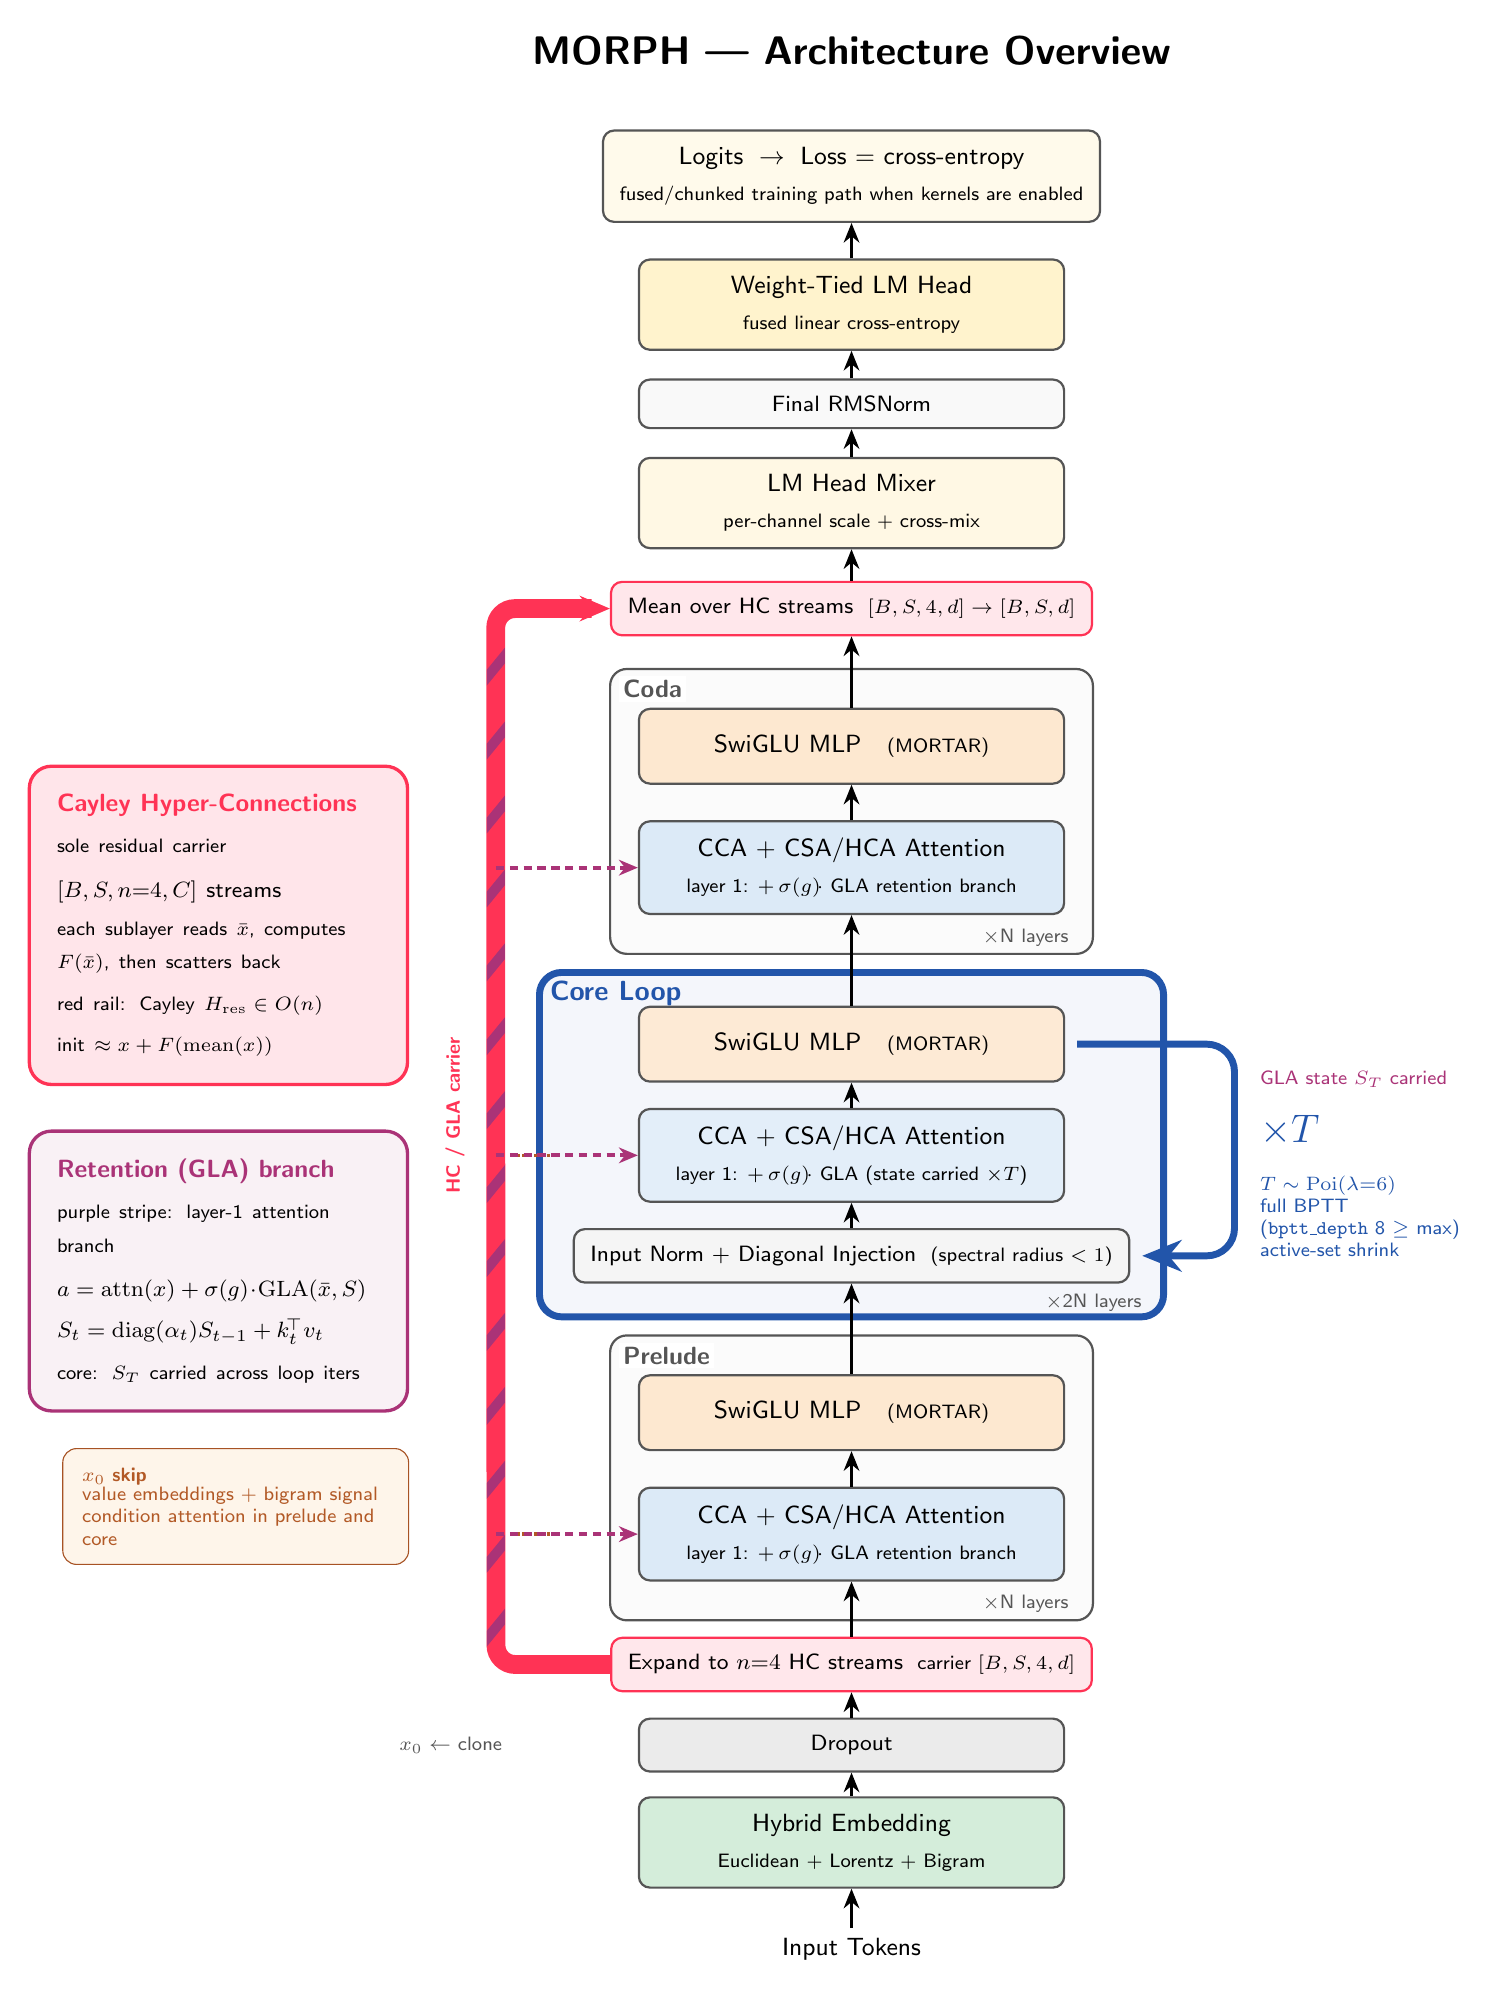
\begin{tikzpicture}[node distance=0.50cm]

% =====================================================================
% MAIN COLUMN (input bottom -> logits top)
% =====================================================================
\node[font=\small\sffamily] (inp) {Input Tokens};

\node[B, fill=fTeal, above=0.5cm of inp] (emb) {
  Hybrid Embedding\\[2pt]{\scriptsize Euclidean + Lorentz + Bigram}};
\draw[A] (inp) -- (emb);

\node[Bs, fill=fGray, above=0.3cm of emb] (drp) {Dropout};
\draw[A] (emb) -- (drp);
\node[sub, text=bdr, left=1.6cm of drp] (x0clone) {$x_0 \leftarrow$ clone};

% ── HC stream expansion ──────────────────────────────────────────────
\node[Bs, fill=hcC!12, draw=hcC, above=0.32cm of drp] (exp) {
  Expand to $n{=}4$ HC streams \;{\scriptsize carrier $[B,S,4,d]$}};
\draw[A] (drp) -- (exp);

% ── PRELUDE ──────────────────────────────────────────────────────────
\node[B, fill=fBlue, above=0.7cm of exp] (pa) {
  CCA + CSA/HCA Attention\\[2pt]
  {\scriptsize layer 1: $+\,\sigma(g)\!\cdot$ GLA retention branch}};
\node[B, fill=fOrange, above=0.45cm of pa] (pm) {SwiGLU MLP\quad{\scriptsize (MORTAR)}};
\draw[A] (exp) -- (pa);
\draw[A] (pa) -- (pm);
\begin{scope}[on background layer]
  \node[draw=bdr, thick, rounded corners=6pt, fill=fGray!20,
        fit=(pa)(pm), inner xsep=10pt, inner ysep=14pt] (PG) {};
\end{scope}
\node[ph, anchor=north west, text=bdr, fill=white, inner sep=1.5pt]
  at ([xshift=0.12cm,yshift=-0.10cm] PG.north west) {Prelude};
\node[sub, text=bdr, anchor=east] at ($(PG.south east)+(-0.2,0.22)$) {$\times$N layers};

% ── CORE LOOP ────────────────────────────────────────────────────────
\node[Bs, fill=fGray!50, above=1.15cm of pm] (inj) {
  Input Norm + Diagonal Injection \;{\scriptsize (spectral radius $<1$)}};
\draw[A] (pm) -- (inj);
\node[B, fill=fBlue!80, above=0.32cm of inj] (ca) {
  CCA + CSA/HCA Attention\\[2pt]
  {\scriptsize layer 1: $+\,\sigma(g)\!\cdot$ GLA (state carried $\times T$)}};
\node[B, fill=fOrange!90, above=0.32cm of ca] (cm) {
  SwiGLU MLP\quad{\scriptsize (MORTAR)}};
\draw[A] (inj) -- (ca);
\draw[A] (ca) -- (cm);
\begin{scope}[on background layer]
  \node[draw=loopC, line width=2.5pt, rounded corners=8pt,
        fill=loopC!5, fit=(inj)(ca)(cm), inner sep=12pt] (CG) {};
\end{scope}
\node[font=\normalsize\sffamily\bfseries, text=loopC, anchor=north west,
      inner sep=1.5pt]
  at ([xshift=0.12cm,yshift=-0.10cm] CG.north west) {Core Loop};
\node[sub, text=bdr, anchor=east] at ($(CG.south east)+(-0.2,0.22)$) {$\times$2N layers};

% loop-back arrow (blue) = the HC carrier + whole block re-applied each iteration
\draw[loopC, line width=2.5pt, rounded corners=10pt,
      -{Stealth[length=5mm,width=4mm]}]
  ($(cm.east)+(0.15,0)$) -- ++(2.0,0) |- ($(inj.east)+(0.15,0)$);
% GLA cross-iteration state carry (Axis 2, retention_carry=true) rides the same loop: annotate above xT
\node[sub, text=cbPurple, anchor=west]
  at ($(cm.east)+(2.35,-0.45)$) {GLA state $S_T$ carried};
\node[font=\Large\sffamily\bfseries, text=loopC, anchor=west]
  at ($(cm.east)+(2.35,-1.1)$) {$\times T$};
\node[sub, text=loopC, align=left, anchor=north west]
  at ($(cm.east)+(2.35,-1.55)$)
  {$T \sim \mathrm{Poi}(\lambda{=}6)$\\full BPTT\\(\texttt{bptt\_depth} 8 $\ge$ max)\\active-set shrink};

% ── CODA ─────────────────────────────────────────────────────────────
\node[B, fill=fBlue, above=1.15cm of cm] (da) {
  CCA + CSA/HCA Attention\\[2pt]
  {\scriptsize layer 1: $+\,\sigma(g)\!\cdot$ GLA retention branch}};
\node[B, fill=fOrange, above=0.45cm of da] (dm) {SwiGLU MLP\quad{\scriptsize (MORTAR)}};
\draw[A] (cm) -- (da);
\draw[A] (da) -- (dm);
\begin{scope}[on background layer]
  \node[draw=bdr, thick, rounded corners=6pt, fill=fGray!20,
        fit=(da)(dm), inner xsep=10pt, inner ysep=14pt] (DG) {};
\end{scope}
\node[ph, anchor=north west, text=bdr, fill=white, inner sep=1.5pt]
  at ([xshift=0.12cm,yshift=-0.10cm] DG.north west) {Coda};
\node[sub, text=bdr, anchor=east] at ($(DG.south east)+(-0.2,0.22)$) {$\times$N layers};

% ── HC collapse + head ───────────────────────────────────────────────
\node[Bs, fill=hcC!12, draw=hcC, above=0.4cm of DG] (col) {
  Mean over HC streams \;{\scriptsize $[B,S,4,d]\to[B,S,d]$}};
\draw[A] (dm) -- (col);

\node[B, fill=fYellow!55, above=0.4cm of col] (mix) {
  LM Head Mixer\\[2pt]{\scriptsize per-channel scale + cross-mix}};
\draw[A] (col) -- (mix);

\node[Bs, fill=fGray!30, above=0.35cm of mix] (fn) {Final RMSNorm};
\draw[A] (mix) -- (fn);

\node[B, fill=fYellow, above=0.35cm of fn] (hd) {
  Weight-Tied LM Head\\[2pt]{\scriptsize fused linear cross-entropy}};
\draw[A] (fn) -- (hd);

\node[B, fill=fYellow!40, above=0.45cm of hd] (out) {
  Logits \;$\to$\; Loss $=$ cross-entropy\\[2pt]
  {\scriptsize fused/chunked training path when kernels are enabled}};
\draw[A] (hd) -- (out);

% =====================================================================
% LEFT: HC CARRIER RAIL + RETENTION BRANCH
% =====================================================================
% Candy-striped carrier rail: red-pink = Cayley HC carrier, purple stripes = GLA side branch.
% It starts when token embeddings expand to n=4 streams, runs in parallel to the backbone,
% then collapses at mean().
\coordinate (hcBot) at ($(exp.west)+(-1.45,0)$);
\coordinate (hcTop) at ($(col.west)+(-1.45,0)$);
\draw[hcC, line width=6.8pt, rounded corners=7pt, -{Stealth[length=3.8mm,width=3.2mm]}]
  (exp.west) -- (hcBot) -- (hcTop) -- (col.west);
% Keep stripes inside the red carrier body. They need to read as thick bands
% without bleeding past the rail edge at preview scale.
\begin{scope}
  \clip ($(hcBot)+(-0.115,0.05)$) rectangle ($(hcTop)+(0.115,-0.05)$);
  \foreach \p in {0.035,0.105,...,0.98}{
    \draw[cbPurple, line width=3.6pt, line cap=butt]
      ($(hcBot)!\p!(hcTop)+(-0.18,-0.22)$) --
      ($(hcBot)!\p!(hcTop)+(0.18,0.22)$);
  }
\end{scope}
\node[font=\scriptsize\sffamily\bfseries, text=hcC, anchor=south, rotate=90]
  at ($(hcBot)!0.52!(hcTop)+(-0.27,0)$) {HC / GLA carrier};

\node[draw=hcC, very thick, rounded corners=8pt, fill=hcFill,
      text width=4.10cm, inner sep=10pt, align=left, anchor=east]
      (HC) at ($(hcBot)!0.70!(hcTop)+(-1.10,0)$) {%
  {\small\sffamily\bfseries\textcolor{hcC}{Cayley Hyper-Connections}}\\[3pt]
  {\scriptsize\sffamily sole residual carrier}\\[4pt]
  {\footnotesize\sffamily $[B,S,n{=}4,C]$ streams}\\[2pt]
  {\scriptsize\sffamily each sublayer reads $\bar{x}$, computes $F(\bar{x})$, then scatters back}\\[3pt]
  {\scriptsize\sffamily red rail: Cayley $H_{\mathrm{res}}\in O(n)$}\\[3pt]
  {\scriptsize\sffamily init $\approx x+F(\mathrm{mean}(x))$}};

\node[draw=cbPurple, very thick, rounded corners=8pt, fill=cbPurple!7,
      text width=4.10cm, inner sep=10pt, align=left, anchor=north east]
      (GLAP) at ($(HC.south east)+(0,-0.55)$) {%
  {\small\sffamily\bfseries\textcolor{cbPurple}{Retention (GLA) branch}}\\[3pt]
  {\scriptsize\sffamily purple stripe: layer-1 attention branch}\\[4pt]
  {\footnotesize\sffamily $a=\mathrm{attn}(x)+\sigma(g)\!\cdot\!\mathrm{GLA}(\bar{x},S)$}\\[3pt]
  {\footnotesize\sffamily $S_t=\mathrm{diag}(\alpha_t)S_{t-1}+k_t^{\!\top}v_t$}\\[3pt]
  {\scriptsize\sffamily core: $S_T$ carried across loop iters}};

% x0 skip is a static conditioning path into attention; use one quiet note and
% subtle orange ticks instead of long cross-page arrows.
\node[draw=cbOrange!70!black, rounded corners=5pt, fill=fOrange!45,
      text width=3.9cm, inner sep=7pt, align=left,
      font=\scriptsize\sffamily, text=cbOrange!75!black, anchor=north east]
      (x0note) at ($(GLAP.south east)+(0,-0.45)$) {%
  \textbf{$x_0$ skip}\\[-1pt]
  value embeddings + bigram signal condition attention in prelude and core};
\foreach \attn in {pa,ca}{
  \draw[cbOrange!75!black, line width=1.2pt, densely dotted]
    ($(hcBot |- \attn.west)+(0.18,0)$) -- ++(0.52,0);
}

% Only layer-1 attention receives the purple side branch.
\foreach \attn in {pa,ca,da}{
  \draw[GLA] (hcBot |- \attn.west) -- (\attn.west);
}

% ── Title ────────────────────────────────────────────────────────────
\node[above=0.7cm of out, font=\Large\sffamily\bfseries]
  {MORPH --- Architecture Overview};

\end{tikzpicture}
\end{document}
